% !Mode:: "TeX:UTF-8"
% !TEX program  = xelatex

%\documentclass{cumcmthesis}
\documentclass[withoutpreface,bwprint]{cumcmthesis} %去掉封面与编号页,电子版提交的时候使用。


\usepackage[framemethod=TikZ]{mdframed}
\usepackage{url}   % 网页链接
\usepackage{subcaption} % 子标题
\title{基于MATLAB的回流焊炉温曲线优化研究}
\tihao{A}
\baominghao{202001002059}
\schoolname{清华大学}
\membera{朱菁菁}
\memberb{陶乐天}
\memberc{向启步}
\supervisor{梁恒}
\yearinput{2020}
\monthinput{09}
\dayinput{12}

\begin{document}

 \maketitle
 \begin{abstract}
 本文针对回焊炉工作过程中焊接区域的升温情形进行建模分析。先对题目附件提供的已知回焊炉的工作状态下焊接区域的温度变化情况进行曲线拟合。然后在该工作状态下,通过能量守恒与Fourier定律,对炉中空气温度的一维分布建立热传导微分方程,并结合边界条件进行求解。再通过对元件厚度方向建立热传导微分方程,考虑空气对流,利用牛顿冷却定律求解边界条件,而热扩散系数等未知量先通过查阅资料以获得数值的大致数量级,然后通过细化步长,在边界条件变化的情况下,使用向前差分法进行空间离散化,再利用matlab进行迭代求解。将模型求解得到的结果与实际附件提供的曲线进行差值比较,以其差值在各点为零为目标进行模型优化。得到未知的热扩散系数与最优模型解。
 
 问题一,由于只能改变外部条件,所以只需要将新的外部条件输入模型,以得到最终结果。
 
 问题二,同样是给定了小温区温度,但是对传送带速度进行规划。绘制出炉温曲线之后,利用制程界限对炉温曲线进行筛选。最终求解得到的最大传送带速度是$\textbf{85cm/min}$。
 
 问题三,由于温区与传送带速度都是待定,所以需要对小温区温度与传送带速度进行有筛选的遍历,分别计算出不同条件下阴影部分的面积,然后找出最小值时的各小温区温度与传送带速度。在探究了基本遍历之后,又思考并实现了粒子群算法,直接全局搜索找到最小的阴影面积与相应的环境因素。
 
 问题四,对最优曲线添加了在$217^{\circ}C$以上以峰值为中心线尽量对称的条件限制,结合问题三,可用峰值左右面积之差$\Delta S$尽量小作为对称判据,以左右面积之差$\Delta S$作为适应值,再次进行粒子群算法,得出面积之差最小时,相应的环境因素。要求面积的之差最小,那相应的面积基值也会变小。因此可以认为是建立在问题三的基础上得到的结果。
 
\keywords{微分方程模型\quad  有限向前差分法\quad   粒子群算法\quad 炉温曲线\quad  制程界限}
\end{abstract}



%目录  2019 明确不要目录,我觉得这个规定太好了
%\tableofcontents

%\newpage

\section{问题重述}
回焊炉实际上就是给电路板进行加热的一个通道,通过传送带将电路板从炉前区域,运送通过预热区、恒温区、回流区等区域进行加热,然后通过冷却区降温。本题就旨在研究整个过程中焊接区域处的热量传导与温度变化问题。温度传感器可以测得焊接区域中心的温度,然后得到炉温曲线。而在焊接生产中,炉温曲线需要满足一定的要求,被称为制程界限。
\begin{flushleft}
\textbf{问题一:}
\end{flushleft}

请对焊接区域的温度变化规律建立数学模型。假设传送带过炉速度为78 cm/min,各温区温度的设定值分别为$173^{\circ}C$(小温区1$\sim$5)、$198^{\circ}C$(小温区6)、$230^{\circ}C$(小温区7)和$257^{\circ}C$(小温区8$\sim$9),请给出焊接区域中心的温度变化情况,列出小温区3、6、7中点及小温区8结束处焊接区域中心的温度,画出相应的炉温曲线,并将每隔$0.5s$焊接区域中心的温度存放在提供的result.csv中。

\begin{flushleft}
	\textbf{问题二:}
\end{flushleft}

假设各温区温度的设定值分别为$182^{\circ}C$(小温区1$\sim$5)、$203^{\circ}C$(小温区6)、$237^{\circ}C$(小温区7)、$254^{\circ}C$(小温区8$\sim$9),请确定允许的最大传送带过炉速度。

\begin{flushleft}
	\textbf{问题三:}
\end{flushleft}

在焊接过程中,焊接区域中心的温度超过$217^{\circ}C$的时间不宜过长,峰值温度也不宜过高。理想的炉温曲线应使超过$217^{\circ}C$到峰值温度所覆盖的面积(图中阴影部分)最小。请确定在此要求下的最优炉温曲线,以及各温区的设定温度和传送带的过炉速度,并给出相应的面积。

\begin{flushleft}
	\textbf{问题四:}
\end{flushleft}

在焊接过程中,除满足制程界限外,还希望以峰值温度为中心线的两侧超过$217^{\circ}C$的炉温曲线应尽量对称。请结合问题3,进一步给出最优炉温曲线,以及各温区设定的温度及传送带过炉速度,并给出相应的指标值。

\section{问题分析}
\subsection{建模分析} 
问题一要求对焊接区域的温度变化规律建立数学模型。在给定过炉速度,给定各温区温度之后,要求得到焊接区域中心的温度变化情况。由于题目并没有给出回焊炉以及焊接元件的传热相关参数,而是通过附件,提供了一个在已知情况下的炉温曲线。因此此题的目标相对比较明确,及通过热传导的关系,用代定系数的方式得到焊接区域中心的温度变化规律,然后通过附件所给的已知情景,将代定系数确定下来。然后建立起模型。建立该模型需要考虑两个方面,一个是炉内温度的空间分布,另一个是焊接区域的温度随时间变化的关系。

关于炉内温度的空间分布,由于小温区基本上能保持温度不变,需要更多考虑的是间隙以及炉前区域与炉后区域的温度分布。该分布可以通过一维的热传导方程进行求解,由于题目提到,空气在短时间内可以达到稳定,因此热传导方程中,可以认为空间中的某处温度稳定,不随时间的变化而改变。则不同温度的小温区之间的间隙温度分布可以考虑为梯度分布。同样的,炉前区域与炉后区域也可以用相同的方式进行求解。

关于焊接区域的温度随时间的变化,在焊接区域的厚度方向上,先由牛顿冷却公式得到焊接区域表面温度,再以表面温度为边界条件,可以列出热传导方程。而题目中的温度传感器测量的区域为焊接区域的中心位置,所以考虑中心位置处的升温规律。以中心位置处为原点坐标,建立y轴进行分析。将连续微分方程离散化,分别设定合适的时间步长与空间步长,利用向前差分法进行差分迭代,计算并绘制出焊接区域的升温曲线。

\subsection{问题一的分析}
问题一只不过改变了相应的外部输入条件,使得升温的速度以及传送带速度有所改变,但物理模型并没有变化,只需要将外部条件输入即可得到相应的炉温曲线。同时完成题目要求的各个点的温度数值填写。


\subsection{问题二的分析}

对于问题二,同样是给定了小温区温度,但是对传送带速度进行规划。从$65cm/min$开始,以$1cm/min$为步长进行遍历,一直到$100cm/min$,分别进行炉温曲线的绘制,绘制出炉温曲线之后,利用制程界限对炉温曲线进行筛选,符合要求的曲线将被记录下来,并且记录下相应的传送带速度,找出速度的最大值。

\subsection{问题三的分析}
问题三,由于温区与传送带速度都是待定,所以需要对小温区温度与传送带速度进行有筛选的遍历,分别计算出不同条件下阴影部分的面积,然后找出最小值时的各小温区温度与传送带速度。但由于遍历层数较多,计算量会很大,因此可以对影响阴影部分面积的各个因素分别进行拟合,得出其对于阴影面积的影响大小。重点遍历对阴影部分影响更大的几项因数,然后再对其它因素进行微调,以找出最小的阴影面积与相应的环境条件。

而此题由于是考虑最优解问题,因此可以采用粒子群算法,应用于大规模数据的全局最优解的寻找。粒子群算法的基础理论可以理解,任一个体(粒子)皆可用有自身移动过程中所产生的记忆与经验,当个体移动的同时,能依造自身的经验与记忆来学习调整自身的移动方向,由于在粒子群算法中,多个粒子是同时移动的,且同时以自身经验与其他粒子所提供的经验进行比对找寻最适当的解,并使自己处于最适解中。

\subsection{问题四的分析}
问题四,对最优曲线添加了在$217^{\circ}C$以上以峰值为中心线尽量对称的条件限制,结合问题三,可用峰值左右面积之差$\Delta S$尽量小作为对称判据,以左右面积之差$\Delta S$作为适应值,再次进行粒子群算法,得出面积之差最小时,相应的环境因素。要求面积的之差最小,那相应的面积基值也会变小。因此可以认为是建立在问题三的基础上得到的结果。

\section{模型假设}
\begin{enumerate}
	\item 炉间空气在短时间内达到稳定。
	\item 炉前区域之前与炉后区域之后的温度为室温。
	\item 除了小温区以外无其它热源。
	\item 焊接区域的热扩散系数在一定范围内保持不变。
	\item 焊接区域各个方向介质均匀。
	\item 焊接区域各个方向的热传导系数相同。
\end{enumerate}

\newpage
\section{符号说明及名词定义}

\begin{table}[!htb]
	\centering
	\caption{符号说明}
    \begin{tabular}{cc}
        \toprule[1.5pt]
        符号 & 说明\\
        \midrule[1pt]
        $T$ & 温度的一般表述\\
        $x$ & 炉内横向位移\\
        $y$ & 炉内纵向位移\\
        $d$ & 焊接区域厚度\\
        $T_0$ & 室温\\
        $T_{sur}$ & 焊接区域表面温度\\
        $T_{air}(x)$ & 炉内空气温度  \\
        $T_{stannum}(y,t)$ & 焊接区域中心温度 \\
        $T_i$ & 各个小温区的温度\\
        $T^{j}_i$ & 离散化后的焊接区域中心温度\\
        $v$ & 传送带速度 \\
        $t$ & 传送时间 \\
        $k$ & 导热系数 \\
        $c$ & 比热容 \\
        $\rho$ & 密度\\
        $a$ & 合并系数($a=\frac{k}{c\rho}$) \\
        $l_{re}$ & 小温区的距离\\
        $l_{gap}$ & 小温区的间隙距离\\
        $l_{front}$ & 炉前区域的长度\\
        $l_{tail}$ & 炉后区域的长度\\
        
         \bottomrule[1.5pt]
    \end{tabular}
\end{table}

\newpage
\section{模型的建立}
通过热传导的关系,用代定系数的方式得到焊接区域中心的温度变化规律,然后通过附件所给的已知情景,将代定系数确定下来。然后建立起模型。建立该模型需要考虑两个方面,一个是炉内温度的空间分布,另一个是焊接区域的温度随时间变化的关系。
\subsection{炉内空气温度的空间分布}

\subsubsection{热传导公式的推导}
先推导热传导公式。

由能量守恒定理,在物体Ω内任意截取一块D,在时段[$t_1$, $t_2$]上有
\begin{equation}\iiint_{D} c \rho\left(\left.u\right|_{t=t_{2}}-\left.u\right|_{t=t_{1}}\right) d x=-\int_{t_{1}}^{t_{2}} d t \iint_{\mathbb{\partial D}}\!\!\!\!\!\!\!\!\!\!\!\!\!\!\!\!\;\subset\!\supset q \cdot n d S+\int_{t_{1}}^{t_{2}} d t \iiint_{D} \rho f_{0} d x
\end{equation}

u = u(x,t)表示温度分布,c是比热容,ρ是密度,q是热流密度,f0是热 源强度。在dt时段内通过边界∂D中小块dS进入区域的热量 为−q·ndSdt(n为∂D的单位外法向量)。

根据Fourier定律,热流向量与温度梯度成正比(热量流动的原因是在物体内部存在温差),比例k为物体的导热系数
\begin{equation}
q = -k\Delta u
\end{equation}

将Fourier定律代入到能量守恒方程,即得

\begin{equation}\iiint_{D} c \rho\left(\left.u\right|_{t=t_{2}}-\left.u\right|_{t=t_{1}}\right) d x=\int_{t_{1}}^{t_{2}} d t \iint_{\mathbb{\partial D}}\!\!\!\!\!\!\!\!\!\!\!\!\!\!\!\!\;\subset\!\supset k \frac{\partial u}{\partial n} d S+\int_{t_{1}}^{t_{2}} d t \iiint_{D} \rho f_{0} d x
\end{equation}

假设u在柱体Ω×(0,∞)内有连续微商$\frac{\partial u}{\partial t}$,$\frac{\partial ^2 u}{\partial x^2}$,则有
\begin{equation}\int_{t_{1}}^{t_{2}} d t \iiint_{D} c \rho \frac{\partial u}{\partial t} d x=\int_{t_{1}}^{t_{2}} d t \iiint_{D}\left(\nabla \cdot(k \nabla u)+\rho f_{0}\right) d x
\end{equation}

由于传送带在一维的方向进行运动,因此可以将空间分布建立一维分布模型。在忽略其它热源的条件下,可以列出三维热传导方程。
\begin{equation}
\frac{\partial T}{\partial t} - a^2\Delta u = 0
\label{eq:3d}
\end{equation}

将三维热传导方程在一维方向进行简化,得到一维热传导方程。
\begin{equation}
\frac{\partial T}{\partial t} - a^2\frac{\partial ^2T}{\partial x^2} = 0
\label{eq:1d}
\end{equation}

\subsubsection{温度空间分布的求解}
考虑$Dirichlet$边值条件:
\[
	\begin{cases}
	T(0, t) = f(t),\\
	T(l, t) = g(t).
	\end{cases}
\]

下面对一维热导方程进行分析。由于题目假设,回焊炉在启动之后,空气能够迅速地达到稳定,之后焊接工作才开始。所以可以认为,温度$T$与时间$t$无关,则有$\frac{\partial T}{\partial t}=0$,而$a$无法达到无穷大,所以要使得方程\cref{eq:1d}满足,只能是$\frac{\partial ^2T}{\partial x^2} =0$。

所以有$\frac{\partial T}{\partial x} =A$,其中A为常数。可以解得$T = Ax+B$。而$A$与$B$需要通过边值条件进行确定。对于小温区之间的间隙,其边值条件为$T(0, t) = T_i$与$T(l, t) = T_{i+1}$。

当$T_i = T_{i+1}$时,可以解得$T(x, t) = T_i = T_{i+1}$。\\
当$T_i \neq T_{i+1}$时,可以解得$T(x, t) = \frac{T_{i+1}-T_{i}}{\Delta x} x + T_i$。即按照线性变化进行分布。

因此可以先通过简单的分段函数,再结合题目对小温区温度的要示,描述传送带一维方向上的温度分布。
\[
T_{air}(x) = 
\begin{cases}
T_0, & x < 0\\
\frac{T_{1}-T_0}{l_{front}} x + T_0, & 0 \leq x < l_{front}\\
T_1, & l_{front} \leq x < l_{front}+5l_{re} + 4l_{gap}\\
\frac{T_6-T_5}{l_{gap}} (x- (l_{front}+5l_{re} + 4l_{gap})) + T_5, & l_{front}+5l_{re} + 4l_{gap} \leq x < l_{front}+5l_{re} + 5l_{gap}\\
T_6, & l_{front}+5l_{re} + 5l_{gap} \leq x < l_{front}+6l_{re} + 5l_{gap}\\
\frac{T_7-T_6}{l_{gap}} (x- (l_{front}+6l_{re} + 5l_{gap})) + T_6, & l_{front}+6l_{re} + 5l_{gap} \leq x < l_{front}+6l_{re} + 6l_{gap}\\
T_7, & l_{front}+6l_{re} + 6l_{gap} \leq x < l_{front}+7l_{re} + 6l_{gap}\\
\frac{T_8-T_7}{l_{gap}} (x- (l_{front}+7l_{re} + 6l_{gap})) + T_7, & l_{front}+7l_{re} + 6l_{gap} \leq x < l_{front}+7l_{re} + 7l_{gap}\\
T_8, &  l_{front}+7l_{re} + 7l_{gap} \leq x < l_{front}+9l_{re} + 8l_{gap}\\
\frac{T_{10}-T_9}{l_{gap}} (x- (l_{front}+9l_{re} + 8l_{gap})) + T_9, & l_{front}+9l_{re} + 8l_{gap} \leq x < l_{front}+9l_{re} + 9l_{gap}\\
T_{10}. & l_{front}+9l_{re} + 9l_{gap} \leq x < 2l_{front}+11l_{re} + 10l_{gap}\\
\end{cases}
\]

\subsection{焊接区域中心的升温规律}
在焊接区域的厚度方向上,先由牛顿冷却公式,得到焊接区域表面温度。牛顿冷却定律的具体表述为:当物体表面与周围存在温差时,单位时间从单位面积散失的热量与温度差成正比,比例系数为热传导率。

\begin{equation}
\frac{\partial T_{sur}}{\partial t} = K(T_{sur}-T_{air})
\end{equation}

以焊接区域表面温度为边界条件,可以列出热传导方程。而题目中的温度传感器测量的区域为焊接区域的中心位置,所以考虑中心位置处的升温规律。以中心位置处为原点坐标,建立y轴进行分析,如图\ref{fig:hanjiequyu}所示。
\begin{figure}[!h]
	\centering
	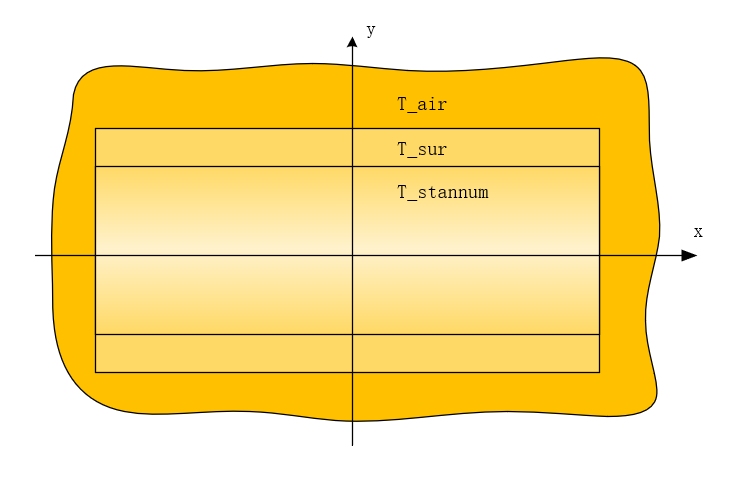
\includegraphics[width=.6\textwidth]{hanjiequyu}
	\caption{焊接区域坐标轴}
	\label{fig:hanjiequyu}
\end{figure}

列出如下方程:
\[
\begin{cases}
\frac{\partial T_{stannum}}{\partial t} - a^2\frac{\partial ^2T_{stannum}}{\partial y^2} = 0, & -\frac{d}{2} < y < \frac{d}{2}, t>0\\
T_{stannum}(-\frac{d}{2}, t) = T_{stannum}(\frac{d}{2}, t) = T_{sur}(vt)\\
T(y, 0) = T_0, & -\frac{d}{2} < y < \frac{d}{2}.\\
\end{cases}
\]

将该连续微分方程离散化,得到
\begin{equation}
T^{j}_0=T(0, jm)=T_{sur}(vt)
\end{equation}
\begin{equation}
T^{j}_n = T(d, jm) = T_{sur}(vt)
\end{equation}
\begin{equation}
T^{0}_i = T(ih, 0) = T_0
\end{equation}

这其中,$m$与$h$分别为时间步长与空间步长。

利用向前差分法,可以得到
\begin{equation}
\frac{T^{j+1}_i-T^{j}_i}{m} = a^2 \frac{T^{j}_{i+1}-2T^{j}_i+T^{j}_{i-1}}{h^2}
\end{equation}

计算得到
\begin{equation}
T^{j+1}_i= sT^{j}_{i+1} + (1-2s)T^{j}_{i}+sT^{j}_{i-1}, \verb|其中|s=\frac{ma^2}{h^2}
\end{equation}

\begin{figure}[!h]
	\centering
	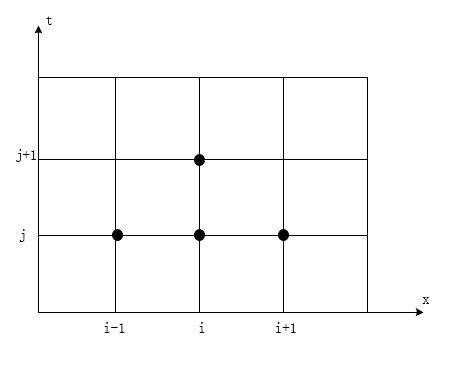
\includegraphics[width=.6\textwidth]{grid}
	\caption{离散网格示意图}
	\label{fig:grid}
\end{figure}

其中,有限差分格式进行计算时是按照时间层逐层推进的。向前差分的离散网格示意图如图\ref{fig:grid}所示。如果考虑二层差分格式,那么计算第i+1层上的值时,需要用到第i层上计算出来的结果值。而计算第i层时的舍入误差(必然会影响到第i+1层的值。所以还需要考虑有限差分法的稳定性。于是需要满足如下的关系:
\begin{equation}
s=\frac{ma^2}{h^2} \leq 0.5
\end{equation}

方便起见,我们固定$s = 0.5$。而$m$与$h$分别根据程序实际取合理步长。


\subsection{模形求解结果}
求解得到焊接区域的温度随时间的变化图像如下图\ref{fig:3D}所示。
\begin{figure}[!h]
	\centering
	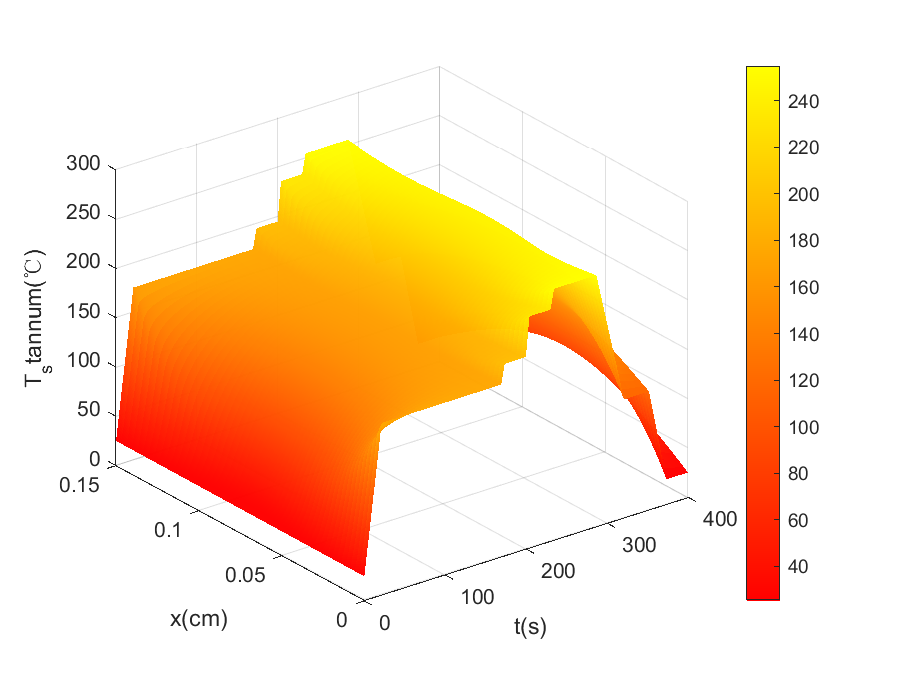
\includegraphics[width=.6\textwidth]{3D}
	\caption{3D模拟模型}
	\label{fig:3D}
\end{figure}

而题目要求监测的是中心点的温度变化曲线,所以在厚度方向上可以取中心点,求得炉温曲线。
\subsubsection{模型1:未修正模型}
跟据查阅的资料可知,a的取值大致为$10^{-3}$量级。通过大致的手动调参,可以得到如图\ref{fig:a}所示建模结果。
\begin{figure}[!h]
	\centering
	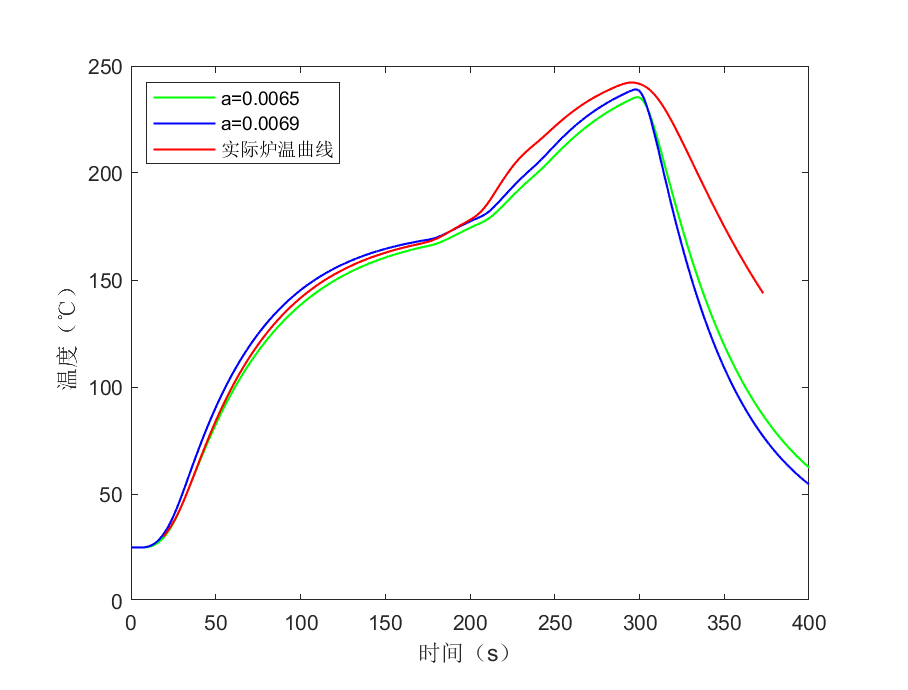
\includegraphics[width=.6\textwidth]{a}
	\caption{模型拟合结果1}
	\label{fig:a}
\end{figure}

当a取值为0.0065与0.00069时,曲线的前170s拟合得十分接近,但之后的上升阶段与峰值之后的下降阶段拟合情况不够理想。可应该需要对模型进行进一步修正。

取a为\textbf{0.0067}。

通过查阅资料,可以了解到,对于一般工业生产使用的焊接材料锡线而言,其加温至$170^{\circ}C$左右时,已经初步出现熔化情况,因此其热扩散系数a可能会有所改变。由于热胀冷缩以及液化的情况,所以材料的密度$\rho$会有较大幅度的降低,相应的,热扩散系数$a = \frac{k}{c\rho}$会有一定程度的升高。

\subsubsection{模型2:热扩散系数修正后的模型}
监测温度节点$T_{stannum}=167^{\circ}C$,当到达该温度后,对模型的热扩散系数进行修正。同样的,通过大致的手动调参,得到如图\ref{fig:a2}所示的建模结果。
\begin{figure}[!h]
	\centering
	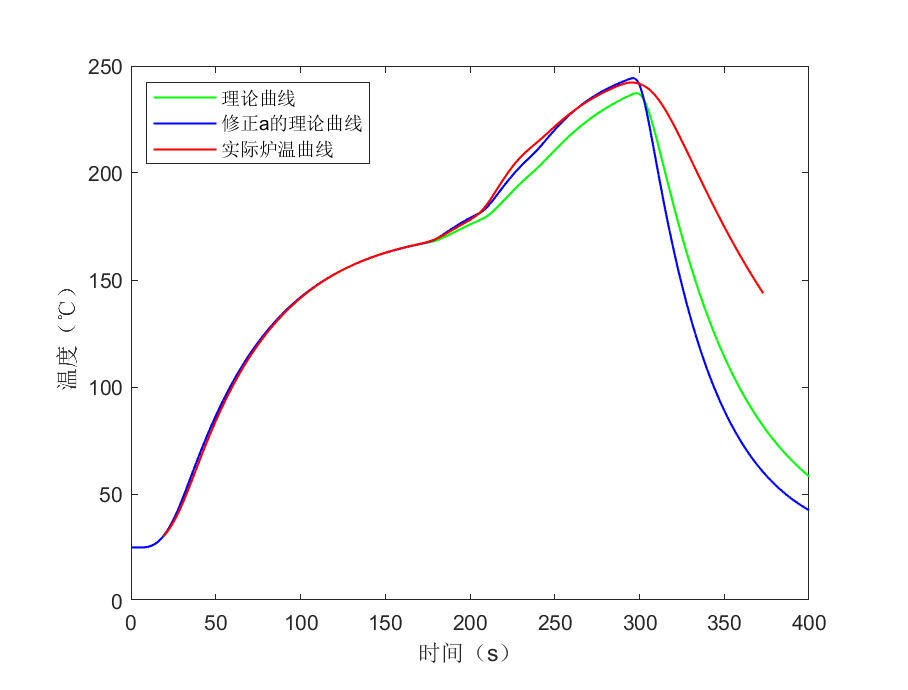
\includegraphics[width=.6\textwidth]{a2}
	\caption{模型拟合结果2}
	\label{fig:a2}
\end{figure}

对$167^{\circ}C$之后的热扩散系数,修正为\textbf{0.0077}时,可以从图中看出,拟合得到的曲线,在上升部分已经与实际曲线重合度很高了。但是峰值之后的下降阶段,依然与实际曲线有较大误差。

\subsubsection{模型3:温区空间分布修正后的模型(最终模型)}
\textbf{于是将修正方案转向空间温度分布模型。}由于题目提示,小温区的边界附近温度会受到旁边小温区温度的影响,所以无法准确地保持在其设定温度下。通过经验分析同样也可以发现,冷却区与其之前的加热区温度相差过大,而其间间隙只有$l_{gap}=5cm$,若按原本的模型运行,其环境温度下降过快。

因此对温区空间分布进行一定的修正。

\begin{enumerate}
	\item 对小温区9的后边界进行修正。
	
	从边界处向前推移$l_{gap}$的距离,使其提早$l_{gap}$就开始进行线性降温。
	\item 对小温区10的前边界进行修正。
	
	从边界处向后推移$6l_{gap}$的距离,使其延后$6l_{gap}$再保持冷却低温。
	\item 将冷却区的低温抬升至$120^{\circ}C$,一直到炉后区域结束。
	
\end{enumerate}

\textbf{得到修正后的温度空间分布分段为:}
\begin{figure}[!h]
	\centering
	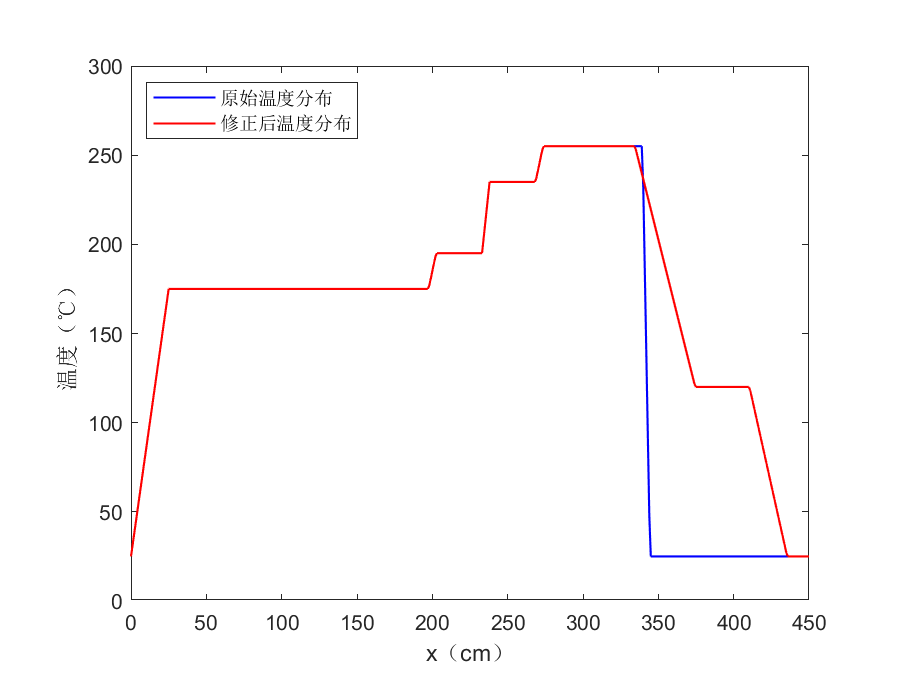
\includegraphics[width=.6\textwidth]{degree}
	\caption{修正后的温度空间分布}
	\label{fig:degree}
\end{figure}

\newpage

在此温度分布下,求得拟合曲线如图\ref{fig:final}所示。
\begin{figure}[!h]
	\centering
	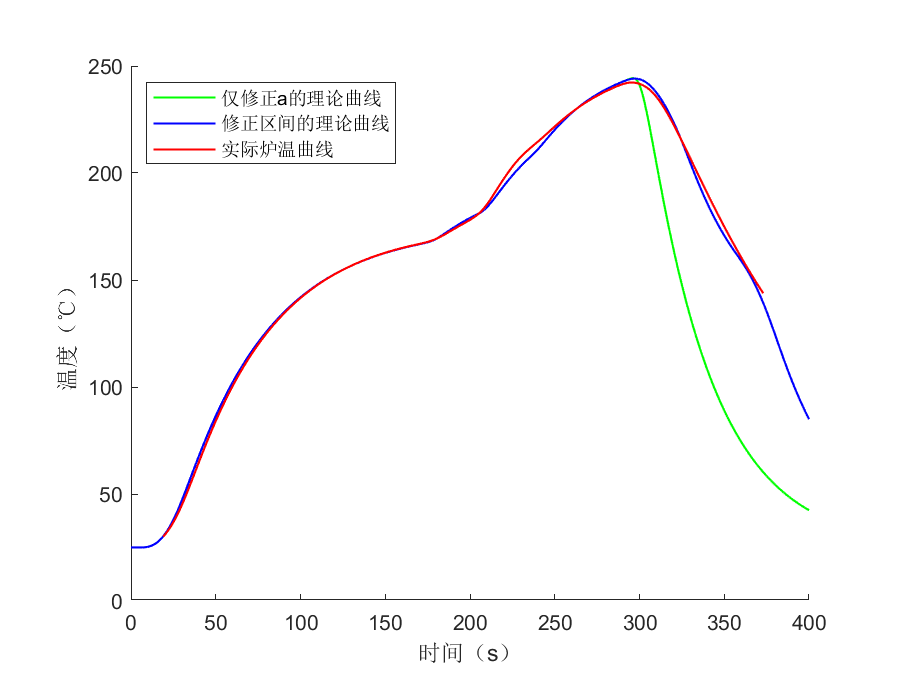
\includegraphics[width=.6\textwidth]{final}
	\caption{模型拟合结果3}
	\label{fig:final}
\end{figure}

从图中可以看出,模型拟合得到的曲线已经与实际曲线基本重合。经过差值比较,画出$\Delta T$的箱形线,如图\ref{fig:xiangxingtu}所示。
\begin{figure}[!h]
	\centering
	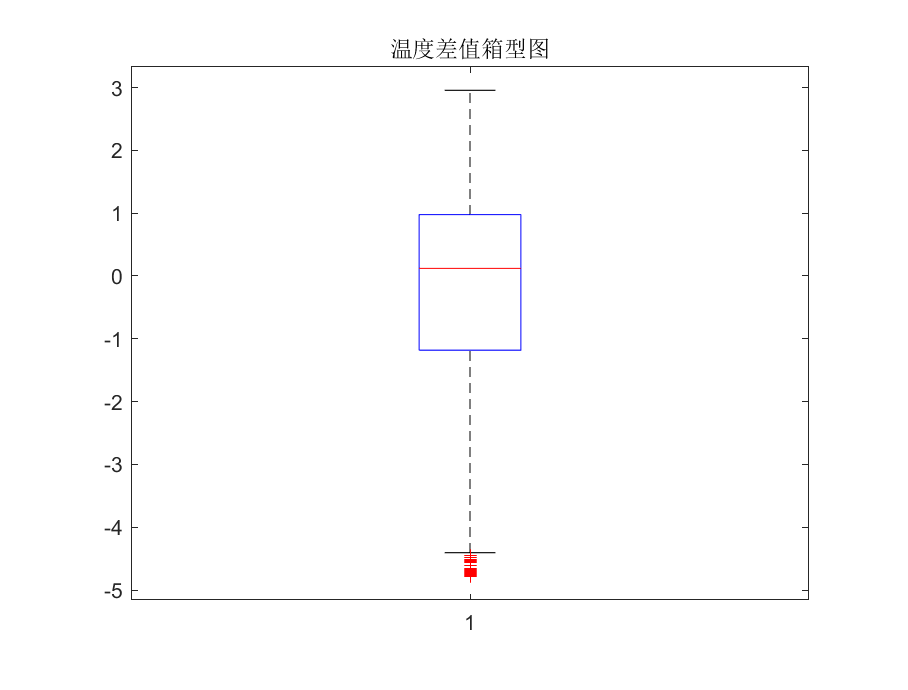
\includegraphics[width=.6\textwidth]{xiangxingtu}
	\caption{温度差值箱形图}
	\label{fig:xiangxingtu}
\end{figure}

找出理论曲线与实际曲线差距最大的两个温度点,$max{\Delta T}=2.9557^{\circ}C$与$min{\Delta T}=-4.7874^{\circ}C$,且中位数为0.12153。基本上能够说明模型的有效性与准确性。

\newpage

\section{问题一的求解}
问题一对模型重新设置了小温区的温度与传送带速度。假设传送带过炉速度为78 cm/min,各温区温度的设定值分别为$173^{\circ}C$(小温区1$\sim$5)、$198^{\circ}C$(小温区6)、$230^{\circ}C$(小温区7)和$257^{\circ}C$(小温区8$\sim$9),请给出焊接区域中心的温度变化情况,列出小温区3、6、7中点及小温区8结束处焊接区域中心的温度,画出相应的炉温曲线,并将每隔$0.5s$焊接区域中心的温度存放在提供的result.csv中。

改变小温区相应的温度曲线,重新运行程序,得到以下炉温曲线。
\begin{figure}[!h]
	\centering
	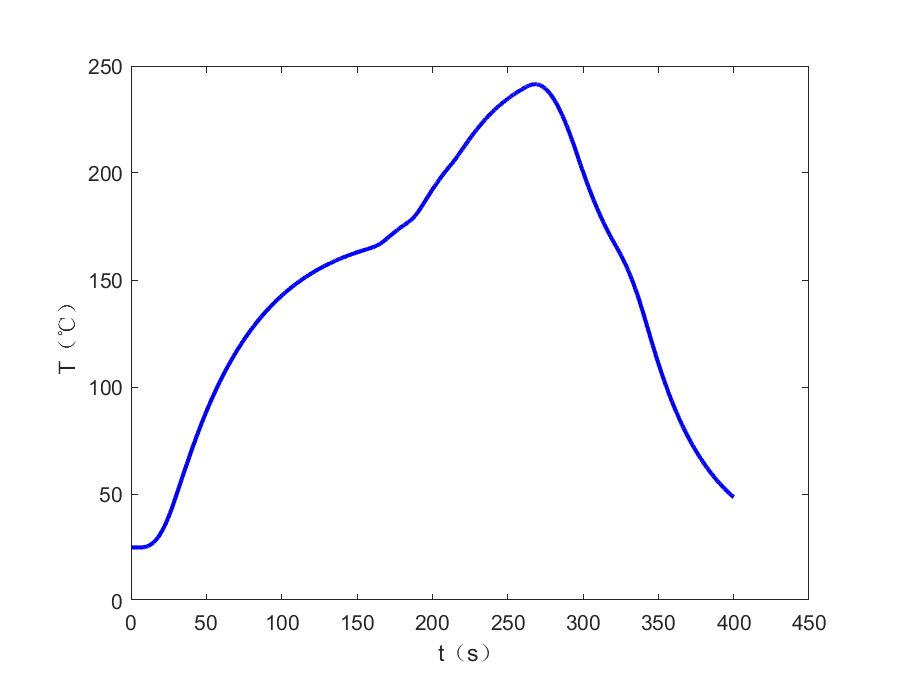
\includegraphics[width=.6\textwidth]{Q1}
	\caption{问题一的炉温曲线}
	\label{fig:Q1}
\end{figure}

并且可以列出小温区3、6、7中点以及小温区8结束处焊接区域中心的温度。
\newpage
\begin{table}[!htb]
	\centering
	\caption{各点的温度}
	\begin{tabular}{cc}
		\toprule[1.5pt]
		温度点 & 温度\\
		\midrule[1pt]
		小温区3中点 & $130.6193^{\circ}C$\\
		小温区6中点 & $166.1973^{\circ}C$\\
		小温区7中点 & $185.7785^{\circ}C$\\
		小温区8结束处 & $223.0759^{\circ}C$\\

		\bottomrule[1.5pt]
	\end{tabular}
\end{table}

相应的具体数据已经存入result.csv中。

\section{问题二的求解}
问题二,同样给出了各温区的温度,速度待定。假设各温区温度的设定值分别为$182^{\circ}C$(小温区1$\sim$5)、$203^{\circ}C$(小温区6)、$237^{\circ}C$(小温区7)、$254^{\circ}C$(小温区8$\sim$9),请确定允许的最大传送带过炉速度。

因此我们可以通过对速度进行遍历,对每一次遍历的炉温曲线,利用制程界限进行筛选,在筛选出符合制程界限的曲线中,找到速度最大的那一条炉温曲线。


求解得到的最大传送带速度是$\textbf{85cm/min}$。


\section{问题三的求解}
\subsection{方案一:整数域内的基本遍历}
基本思路即对各个外部条件进行遍历,从而得到最小的阴影面积。但是考虑到遍历的层数过多,运算量巨大,因而可以先分析各因素对阴影部分影响的程度大小。

当固定传送带速度为$v = 70cm/min$的条件下,由于各个温区的温度变化范围为$\pm10^{\circ}C$,所以用控制变量法,每次只改变一个小温区的温度,探究阴影部分的面积的增长趋势。所得结果如下图所示。
\newpage
\begin{figure}[!h]
	\centering
	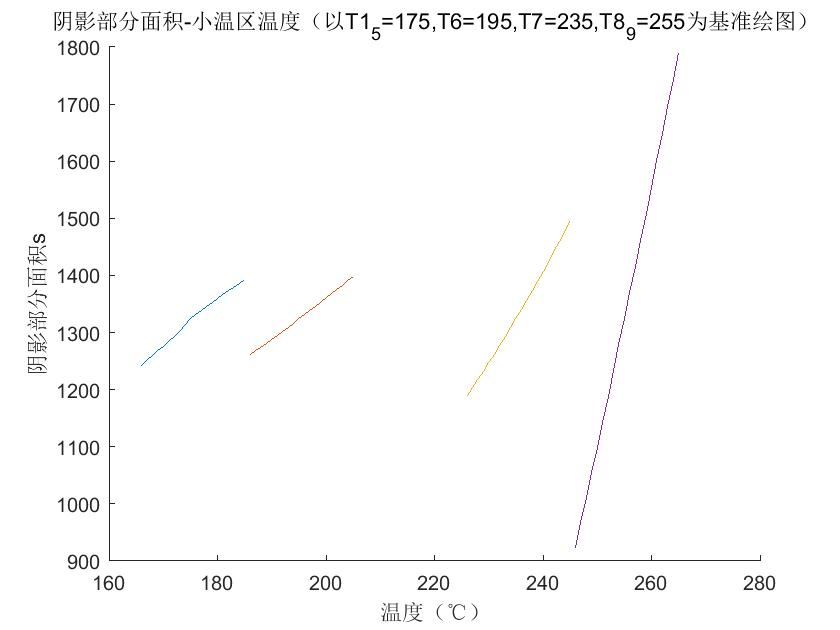
\includegraphics[width=.6\textwidth]{degreeChange}
	\caption{各个温区分别变化时,对阴影部分面积的影响}
	\label{fig:deC}
\end{figure}

从图中可以发现,阴影部分的面积与各小温区的温度之间,基本呈线性变化关系。当温区温度升高,则阴影面积会随之而增大。且可以看出,小温区8、9对阴影部分面积影响最大。同时,分别求出各条直线的斜率,从左至右分别为7.5,6.9,15.35,43.36。因此在遍历搜索最小阴影面积的时候可以重点考虑小温区8、9。

当固定小温区温度为题目所给标准温度时($T_1=175^{\circ}C$,$T_6=195^{\circ}C$,$T_7=235^{\circ}C$,$T_8=255^{\circ}C$),改变传送带的速度,探究阴影部分的面积变化趋势。所得结果如下图所示。
\begin{figure}[!h]
	\centering
	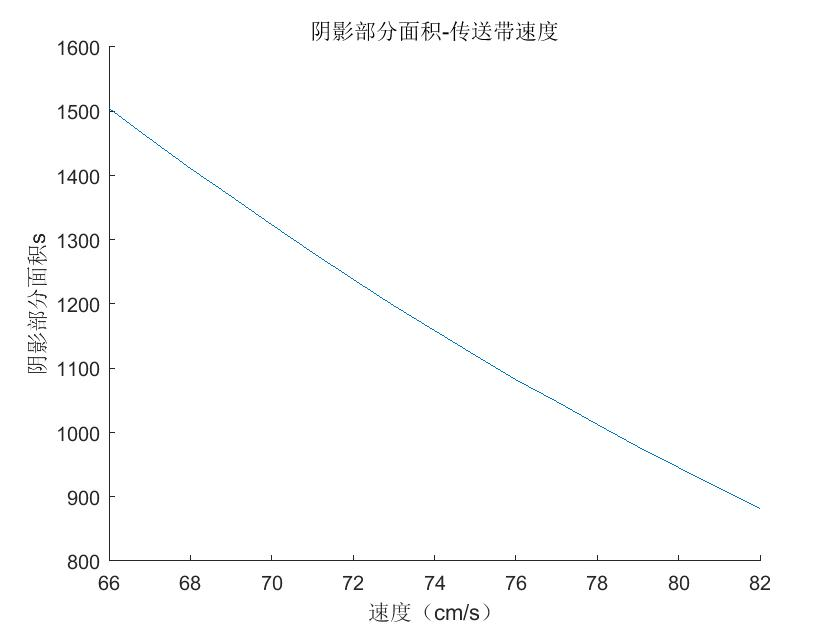
\includegraphics[width=.6\textwidth]{speedChange}
	\caption{传送带速度变化时,对阴影部分面积的影响}
	\label{fig:spC}
\end{figure}

从图中可以发现,阴影部分的面积与传送带速度之间的关系,同样近似为线性关系。当传送带速度越大,则阴影部分面积越小。且用直线拟合之后可以得到其斜率为-88.235。其阴影程度也较大。

综上,在进行遍历求解的过程中,应当对传送带速度与小温区8、9进行较大范围的遍历,对其它小温区可进行较小范围的遍历,这样能够保证运算量适中,且求解结果相对准确。

遍历求解之后得到最小面积为519.23。
且各环境因素分别为
\begin{table}[!htb]
	\centering
	\caption{各环境因素}
	\begin{tabular}{cc}
		\toprule[1.5pt]
		环境因素 & 数值\\
		\midrule[1pt]
		小温区1到5 & $185^{\circ}C$\\
		小温区6 & $205^{\circ}C$\\
		小温区7 & $233^{\circ}C$\\
		小温区8、9 & $255^{\circ}C$\\
		传送带速度 & $87cm/min$\\
		\bottomrule[1.5pt]
	\end{tabular}
\end{table}

在此条件下的最优炉温曲线如下图所示。
\begin{figure}[!h]
	\centering
	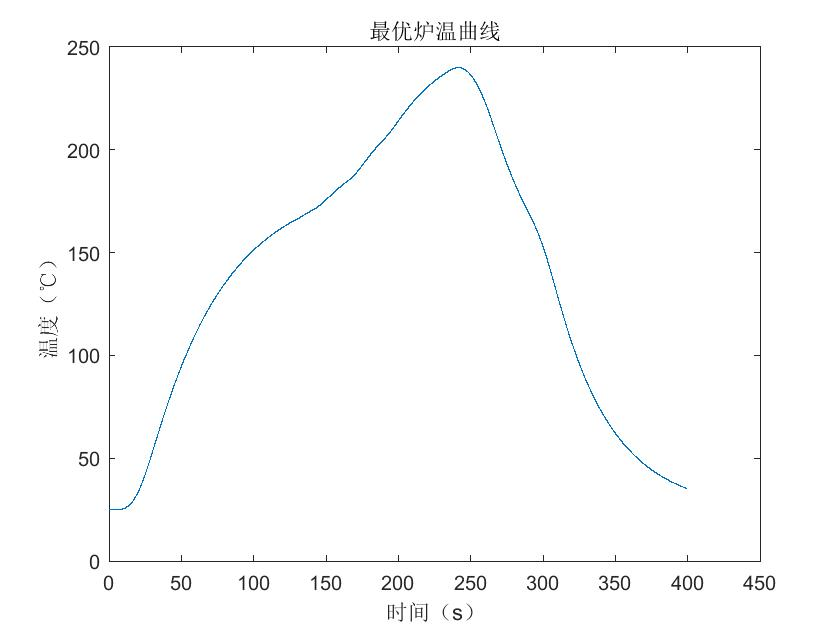
\includegraphics[width=.6\textwidth]{curve_3}
	\caption{此条件下最优炉温曲线}
	\label{fig:cur3}
\end{figure}

\newpage

\subsection{方案二:粒子群算法}
粒子群优化算法(Particle Swarm Optimization,PSO)是一种群智能进化算法,常被应用于大规模数据的全局最优解的寻找,其基本思想是基于鸟类捕食行为中个体对信息的共享,从而使整体向最优解靠近的过程。

首先,假设目标的搜索空间有 D 个维度,初始化 M 个搜索粒子,其中第 i 个粒子当前的位置和速度可以分别表示为:
\begin{equation}
	X_{m}=\left(x_{m 1}, x_{m 2}, \cdots, x_{m D}\right), \quad m=1,2, \cdots, M
\end{equation}


\begin{equation}
	V_{m}=\left(v_{m 1}, v_{m 2}, \cdots, v_{m D}\right), \quad m=1,2, \cdots, M
\end{equation}

在每一次迭代过程中,当单个粒子寻优得到最优适应度值时,记录为个体极值:

\begin{equation}
	p_{\text {best}}=\left(p_{m 1}, p_{m 2}, \cdots, p_{m D}\right), \quad m=1,2, \cdots, M
\end{equation}

当一轮所有粒子的搜索结束后,整个粒子群寻优得到最优位置时,记录为全局极值:

\begin{equation}
	g_{b e s t}=\left(p_{g 1}, p_{g 2}, \cdots, p_{g D}\right)
\end{equation}

接着进行速度和位置的更新:

\begin{equation}
V_{m}^{q+1}=\omega V_{m}^{q}+c_{1} r_{1}\left[X_{g b e s t}-X_{m}^{q}\right]+c_{2} r_{2}\left[X_{p b e s t, m}-X_{m}^{q}\right], \quad m=1,2, \ldots, M
\end{equation}

\begin{equation}
X_{m}^{q+1}=X_{m}^{q}+V_{m}^{q+1}, \quad m=1,2, . ., M
\end{equation}


其中$\omega$为权重因子,$q$为迭代次数,$c_1$, $c_2$分别为表示社会性和个体性的权重因
子,$r_1$, $r_2$为[0,1]范围内的随机数。

这里速度的三项分别表示粒子有维持自身状态的惯性,趋向于群体最优的社
会合作属性,以及朝向自身历史最佳状态的属性,为了能够获得更好的搜索能力,继续采用带有惯性权重的改进粒子群算法。

从前述过程可以看出$\omega$表示粒子保持原有速度状态的权重,而这一点在搜索能力
上就表现出更为优秀的表现。因此$\omega$越大,全局搜索能力越强,局部收敛能力减
弱。

因此如果能在迭代初期采用较大的权重因子,有利于跳出局部最优,便于全
局搜索,而在迭代的后期采用较小的权重因子,从而使得在全局最优点附近较快
收敛,避免振荡现象的出现。可以利用以下公式更改权重因子,其中 t表示当前的迭代步数,$t_{max}$表示总的迭代步数。

\begin{equation}
\omega=\omega_{\max }-\frac{t \times\left(\omega_{\max }-\omega_{\min }\right)}{t_{\max }}
\end{equation}


\begin{figure}[!h]
	\centering
	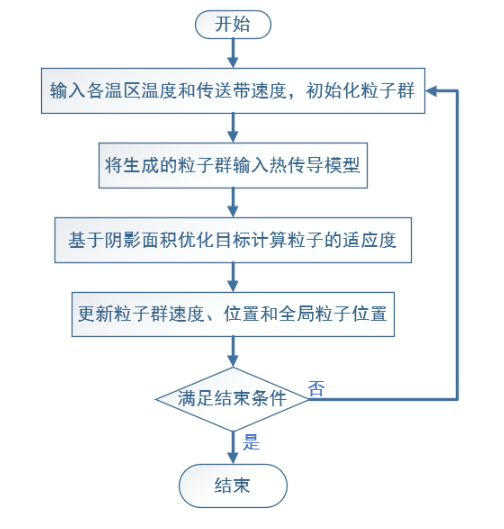
\includegraphics[width=.6\textwidth]{psoliuc}
	\caption{PSO流程图}
	\label{fig:psoliuc}
\end{figure}

在此题中,以阴影部分面积作为适应值。把制程界限以惩罚函数的形式写入适应值。为了简单起见,我们采用常数值作为线性变化权重因子。设置PSO算法的迭代参数,见下表。
\begin{table}[!htb]
	\centering
	\caption{PSO算法的迭代参数}
	\begin{tabular}{cc}
		\toprule[1.5pt]
		参数 & 数值\\
		\midrule[1pt]
		最大迭代次数maxnum & 30\\
		粒子群规模particlesize & 20\\
		个体学习因子$c_1$ & 2\\
		社会学习因子$c_2$ & 2\\
		权重因子$\omega$ & 0.6\\
		\bottomrule[1.5pt]
	\end{tabular}
\end{table}

通过粒子群算法得到的收敛曲线如下图所示。

\newpage
\begin{figure}[!h]
	\centering
	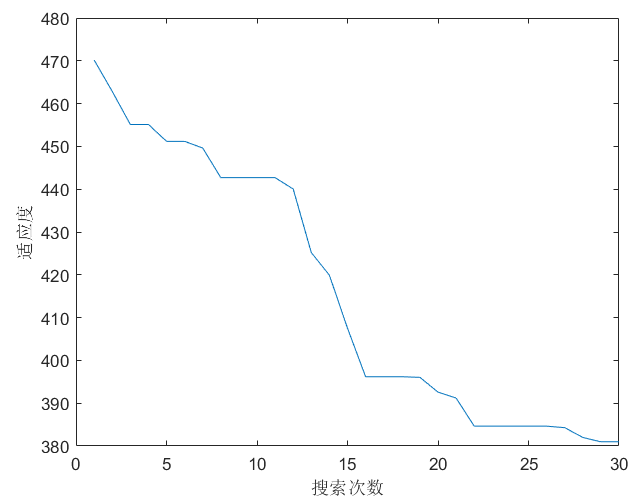
\includegraphics[width=.6\textwidth]{shoulian3}
	\caption{收敛曲线}
	\label{fig:shoulian3}
\end{figure}

粒子群算法求解之后得到最小面积为380.9793。
且各环境因素分别为:
\begin{table}[!htb]
	\centering
	\caption{粒子群算法求解的各环境因素}
	\begin{tabular}{cc}
		\toprule[1.5pt]
		环境因素 & 数值\\
		\midrule[1pt]
		小温区1到5 & $173.400638830053^{\circ}C$\\
		小温区6 & $188.876314235824^{\circ}C$\\
		小温区7 & $231.154182130492^{\circ}C$\\
		小温区8、9 & $ 264.293336606147^{\circ}C$\\
		传送带速度 & $95.1991162503285cm/min$\\
		\bottomrule[1.5pt]
	\end{tabular}
\end{table}

\textbf{可以看出,在粒子群算法计算出来的最小阴影面积比之之前的基本遍历,面积更小。因此更加准确。}

在此条件下的最优炉温曲线如下图所示。
\begin{figure}[!h]
	\centering
	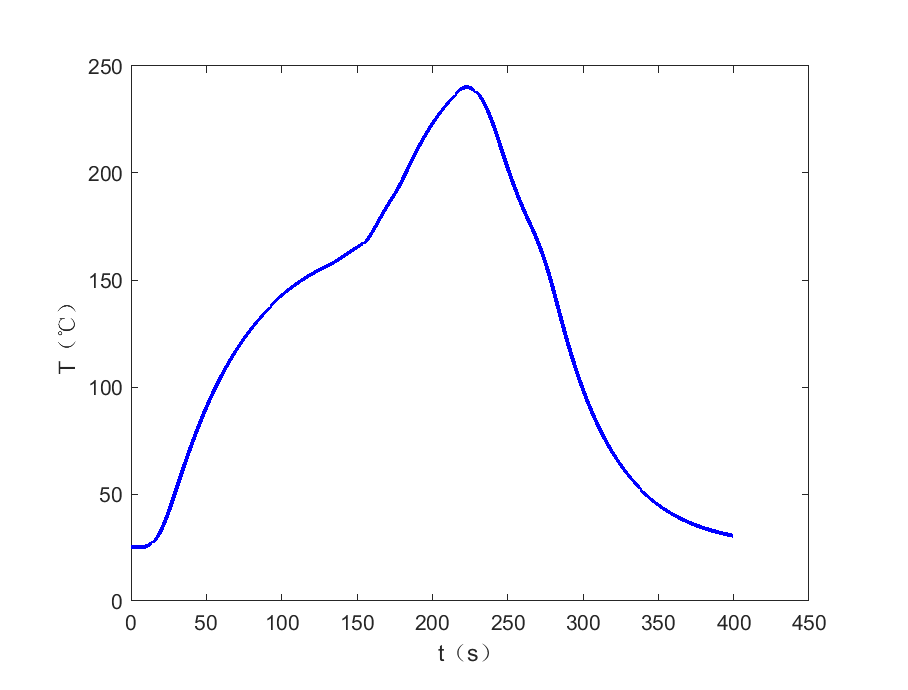
\includegraphics[width=.6\textwidth]{curve_33}
	\caption{此条件下最优炉温曲线}
	\label{fig:cur33}
\end{figure}
\newpage

\section{问题四的求解}
问题四,对最优曲线添加了在$217^{\circ}C$以上以峰值为中心线尽量对称的条件限制,结合问题三,可用峰值左右面积之差$\Delta S$尽量小作为对称判据,以左右面积之差$\Delta S$作为适应值,再次进行粒子群算法,得出面积之差最小时,相应的环境因素。要求面积的之差最小,那相应的面积基值也会变小。因此可以认为是建立在问题三的基础上得到的结果。

在此题中,以左右面积之差$\Delta S$作为适应值。把制程界限以惩罚函数的形式写入适应值。
设置PSO算法的迭代参数。

\begin{table}[!h]
	\centering
	\caption{PSO算法的迭代参数}
	\begin{tabular}{cc}
		\toprule[1.5pt]
		参数 & 数值\\
		\midrule[1pt]
		最大迭代次数maxnum & 30\\
		粒子群规模particlesize & 20\\
		个体学习因子$c_1$ & 2\\
		社会学习因子$c_2$ & 2\\
		权重因子$\omega$ & 0.6\\
		\bottomrule[1.5pt]
	\end{tabular}
\end{table}

通过粒子群算法得到的面积之差的收敛曲线如下图所示。
\newpage
\begin{figure}[!h]
	\centering
	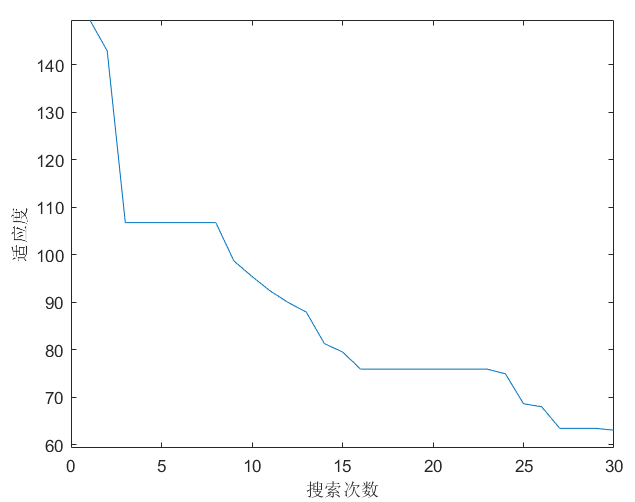
\includegraphics[width=.6\textwidth]{shoulian4}
	\caption{收敛曲线}
	\label{fig:shoulian4}
\end{figure}

粒子群算法求解之后得到最小面积之差为63.1109。因此可以认为最峰值两端对称。

且各环境因素分别为:

\begin{table}[!h]
	\centering
	\caption{此题下各环境因素}
	\begin{tabular}{cc}
		\toprule[1.5pt]
		环境因素 & 数值\\
		\midrule[1pt]
		小温区1到5 & $174.817965172342^{\circ}C$\\
		小温区6 & $190.575404521235^{\circ}C$\\
		小温区7 & $225^{\circ}C$\\
		小温区8、9 & $265^{\circ}C$\\
		传送带速度 & $95.2534787571562cm/min$\\
		\bottomrule[1.5pt]
	\end{tabular}
\end{table}

在此条件下的最优炉温曲线如下图所示。
\newpage
\begin{figure}[!h]
	\centering
	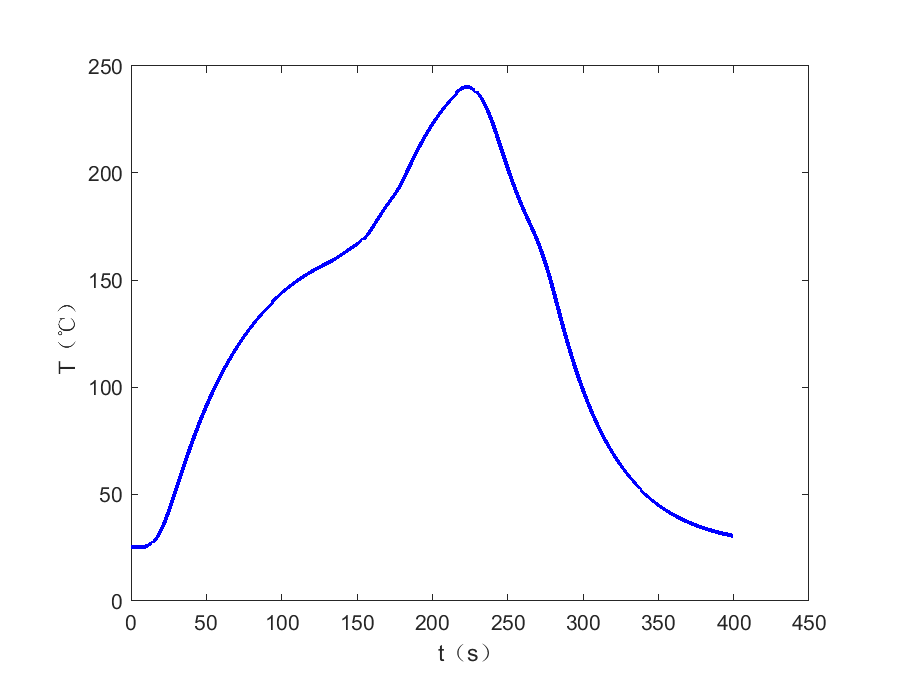
\includegraphics[width=.6\textwidth]{curve4}
	\caption{此条件下最优炉温曲线}
	\label{fig:cur4}
\end{figure}


\newpage
\section{参考文献与引用}

%参考文献
\begin{thebibliography}{9}%宽度9
    \bibitem[1]{mathematical-modeling}
    徐梓斌,闵剑青.基于pdetool的热传导数值计算[J].佳木斯大学学报(自然科学版),2006(02):270-272.
    \bibitem[2]{mathematical-modeling}
    李灿,高彦栋,黄素逸.热传导问题的MATLAB数值计算[J].华中科技大学学报(自然科学版),2002(09):91-93.
    \bibitem[3]{mathematical-modeling}
    阴小波,张磊.浅谈数学建模中的组队和分工技巧[J].科技信息,2010,(23):709.
    \bibitem[4]{mathematical-modeling}
    粒子群优化算法(PSO) \url{https://blog.csdn.net/weixin_40679412/article/details/80571854}
    \bibitem[5]{mathematical-modeling}
    潘峰,李位星,高琪等著. 粒子群优化算法与多目标优化. 北京:北京理工大学出版社, 2013.08.
    \bibitem[6]{mathematical-modeling}
    张天孙主编;郝丽芬编写. 传热学. 北京:中国电力出版社, 2006.02.
\end{thebibliography}

\newpage
%附录
\begin{appendices}
\section{部分关键代码}
\subsection{基本参数设置}


\begin{lstlisting}[language=matlab]
%基本参数设置
%长度
L=30.5; %小温区长度cm
global a
a=5; %间隙cm
ll=25; %炉前区和炉后区长度cm
global d
d=0.15; %焊接区域厚度mm
%各区域温度
global T0
T0=25; %车间温度、炉前区域和炉后区域、10_11保持25度
%可控参数
global v T1_5 T6 T7 T8_9
T1_5=175; %175\pm10
T6=195; %195\pm10
T7=235; %235\pm10
T8_9=255; %255\pm10

%%
%附件炉温曲线
data_raw=readtable('.\附件.xlsx');%将附件添加到当前路径
plot(data_raw{:,1},data_raw {:,2});
title("附件炉温曲线");
xlabel("时间(s)");
ylabel("温度(℃)");


%%
%时间温度分布
hold on
T_temp=zeros(1,400);
v=70; %65_100 cm/min
for i=1:800
T_step(1,i)=temperature_air(i*0.5,v);%以0.5℃为升温梯度
end
plot(0.5:0.5:400,T_step(1,:));
 \end{lstlisting}
 
\subsection{问题一代码}
\begin{lstlisting}[language=matlab]
%问题一
T1_5=173; %175\pm10
T6=198; %195\pm10
T7=230; %235\pm10
T8_9=257; %255\pm10
v=78;
[T,T3,t,t3,N]=get_sol(v);
T_solve=T3(fix(N/2),:)';
plot(t3,T_solve);
title("当前温度下焊接区域中心温度变化情况");
xlabel("时间(s)");
ylabel("温度(℃)");
s3=111.25;
s6=217.75;
s7=253.25;
s8=304;
t_block3=s3/(v/60);
t_block6=s6/(v/60);
t_block7=s7/(v/60);
t_block8=s8/(v/60);
T_blockq=interp1(t3,T_solve',[t_block3,t_block6,t_block7,t_block8]);
T_block3=T_blockq(1)%小温区3中心焊接区域中心的温度
T_block6=T_blockq(2)%小温区6中心焊接区域中心的温度
T_block7=T_blockq(3)%小温区7中心焊接区域中心的温度
T_block9=T_blockq(4)%小温区8结束处焊接区域中心的温度
\end{lstlisting}

\subsection{问题二代码}
\begin{lstlisting}[language=matlab]
v_test=65:1:100; %传送带的速度范围
time=0:0.5:400;
v_able=zeros(1,length(v_test));
for n=1:length(v_able)%传送带的速度范围
flag=1;
v=v_test(n);
T1_5=183; %175\pm10
T6=203; %195\pm10
T7=237; %235\pm10
T8_9=254; %255\pm10
[T,T3,t,t3,N]=get_sol(v);

time=0:0.5:400;
T_solve=interp1(t3,T3(fix(N/2),:),time);
T_solve=T_solve';
%可控参数
T_p=max(T_solve);%峰值温度
T_pp(n)=T_p;
derivative_T=diff(T_solve)/0.5;%温度变化斜率
search=logical(derivative_T>=0);
T_up=derivative_T(search);%温度上升斜率
derivative_T(search)=[];
T_down=derivative_T;%温度下降斜率
dsolve=diff(T_solve);
t_limit=find(T_solve==T_p);
t_low=find(T_solve>=150);
tt_low=find(t_low<t_limit);
t_high=find(ceil(T_solve)<=190);
tt_high=find(t_high<t_limit);
t_dur=max(time(t_high(tt_high)))-min(time(t_low(tt_low)));%温度上升过程中在150℃-190℃的时间
t_217=find(floor(T_solve)>=217);
t_dur217=max(time(t_217))-min(time(t_217));%温度大于217℃的时间;
tt_dur217(n)=t_dur217;

if (max(T_up)>3|min(T_down)<-3|t_dur<60|t_dur>120|t_dur217<40|t_dur217>90|T_p<240|T_p>250)
flag=0;
end

if (flag==1)
v_able(n)=v_test(n);
end

end
v_max=max(v_able);%确定允许的最大传送带过炉速度
\end{lstlisting}

\subsection{PSO关键代码}
\begin{lstlisting}[language=matlab]

v_test=65:1:100; %传送带的速度范围
time=0:0.5:400;
v_able=zeros(1,length(v_test));
for n=1:length(v_able)%传送带的速度范围
flag=1;
v=v_test(n);
T1_5=183; %175\pm10
T6=203; %195\pm10
T7=237; %235\pm10
T8_9=254; %255\pm10
[T,T3,t,t3,N]=get_sol(v);

time=0:0.5:400;
T_solve=interp1(t3,T3(fix(N/2),:),time);
T_solve=T_solve';
%可控参数
T_p=max(T_solve);%峰值温度
T_pp(n)=T_p;
derivative_T=diff(T_solve)/0.5;%温度变化斜率
search=logical(derivative_T>=0);
T_up=derivative_T(search);%温度上升斜率
derivative_T(search)=[];
T_down=derivative_T;%温度下降斜率
dsolve=diff(T_solve);
t_limit=find(T_solve==T_p);
t_low=find(T_solve>=150);
tt_low=find(t_low<t_limit);
t_high=find(ceil(T_solve)<=190);
tt_high=find(t_high<t_limit);
t_dur=max(time(t_high(tt_high)))-min(time(t_low(tt_low)));%温度上升过程中在150℃-190℃的时间
t_217=find(floor(T_solve)>=217);
t_dur217=max(time(t_217))-min(time(t_217));%温度大于217℃的时间;
tt_dur217(n)=t_dur217;

if (max(T_up)>3|min(T_down)<-3|t_dur<60|t_dur>120|t_dur217<40|t_dur217>90|T_p<240|T_p>250)
flag=0;
end

if (flag==1)
v_able(n)=v_test(n);
end

end
v_max=max(v_able);%确定允许的最大传送带过炉速度
\end{lstlisting}
\end{appendices}

\end{document} 